\begin{figure}[tbp]
\centering
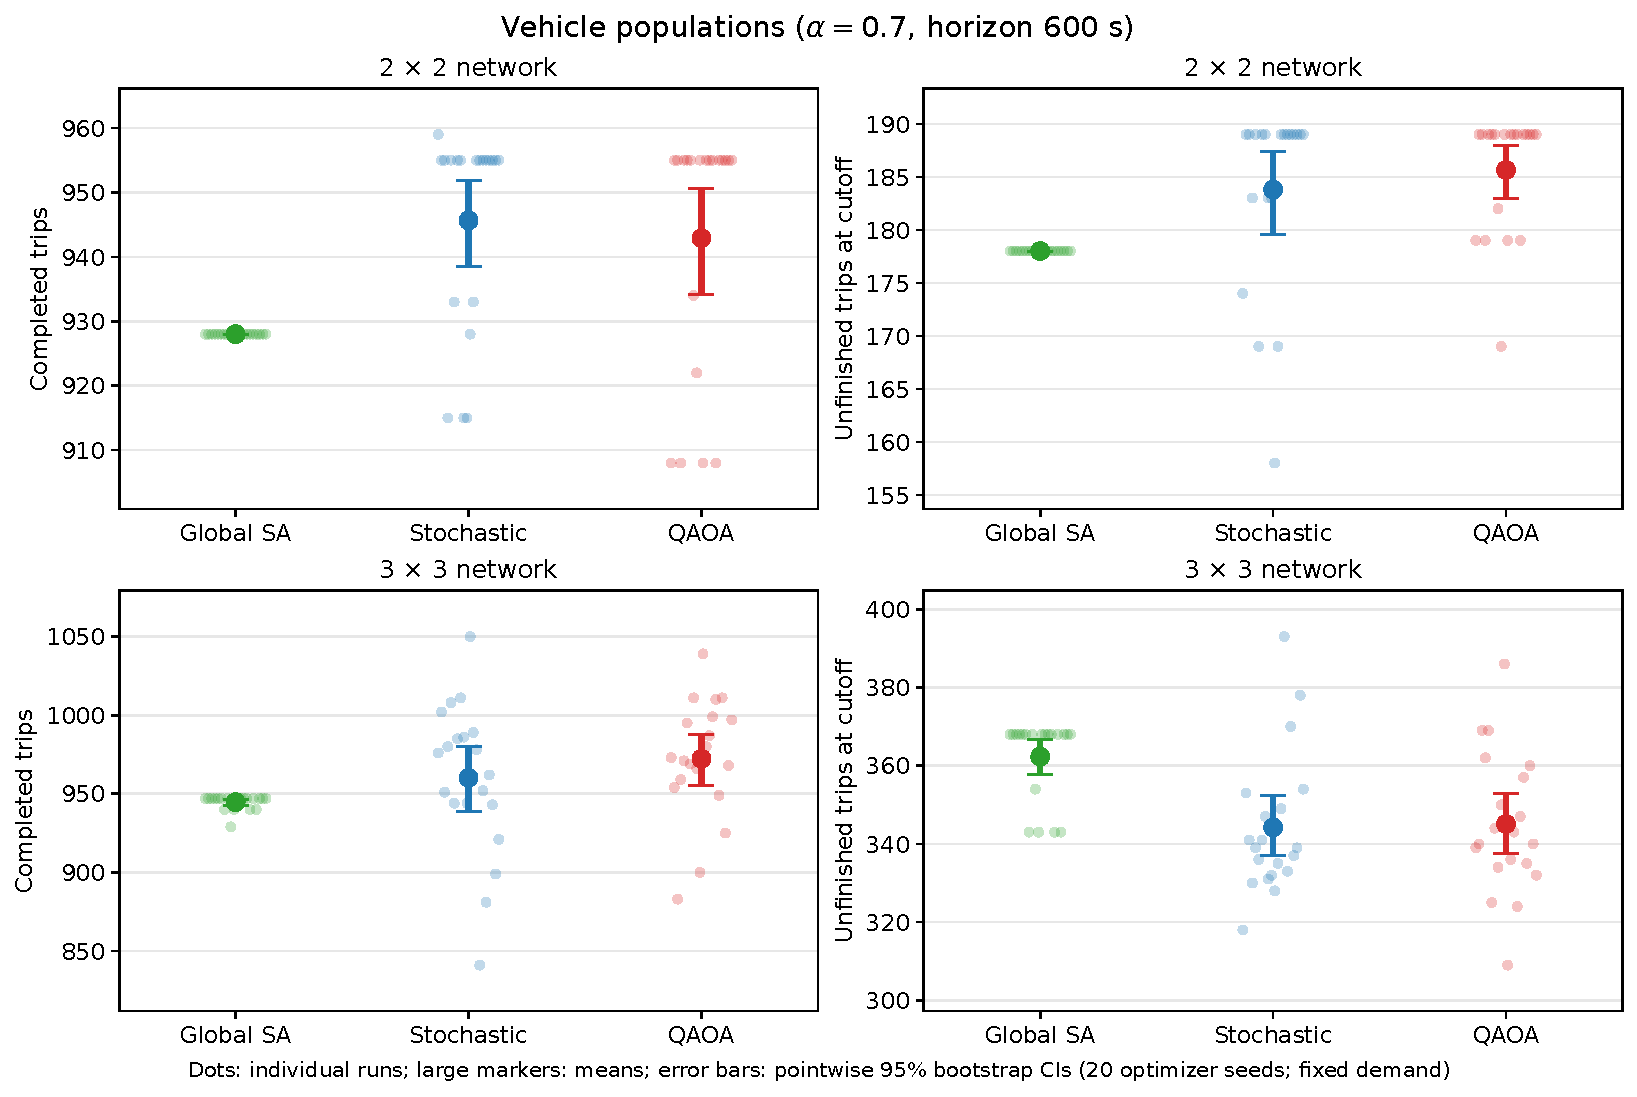
\includegraphics[width=\linewidth]{graphs/reviewer_population_accounting/figure_population.pdf}
\caption{Completed and unfinished vehicle populations at the 600-s cutoff. All conditions use $\alpha=0.7$ and fixed demand. Small dots show individual optimizer runs; large markers show means and error bars show pointwise 95\% percentile-bootstrap confidence intervals across 20 optimizer runs. These are not confidence intervals for controller differences.}
\label{fig:supplementary-population}
\end{figure}

\begin{figure}[tbp]
\centering
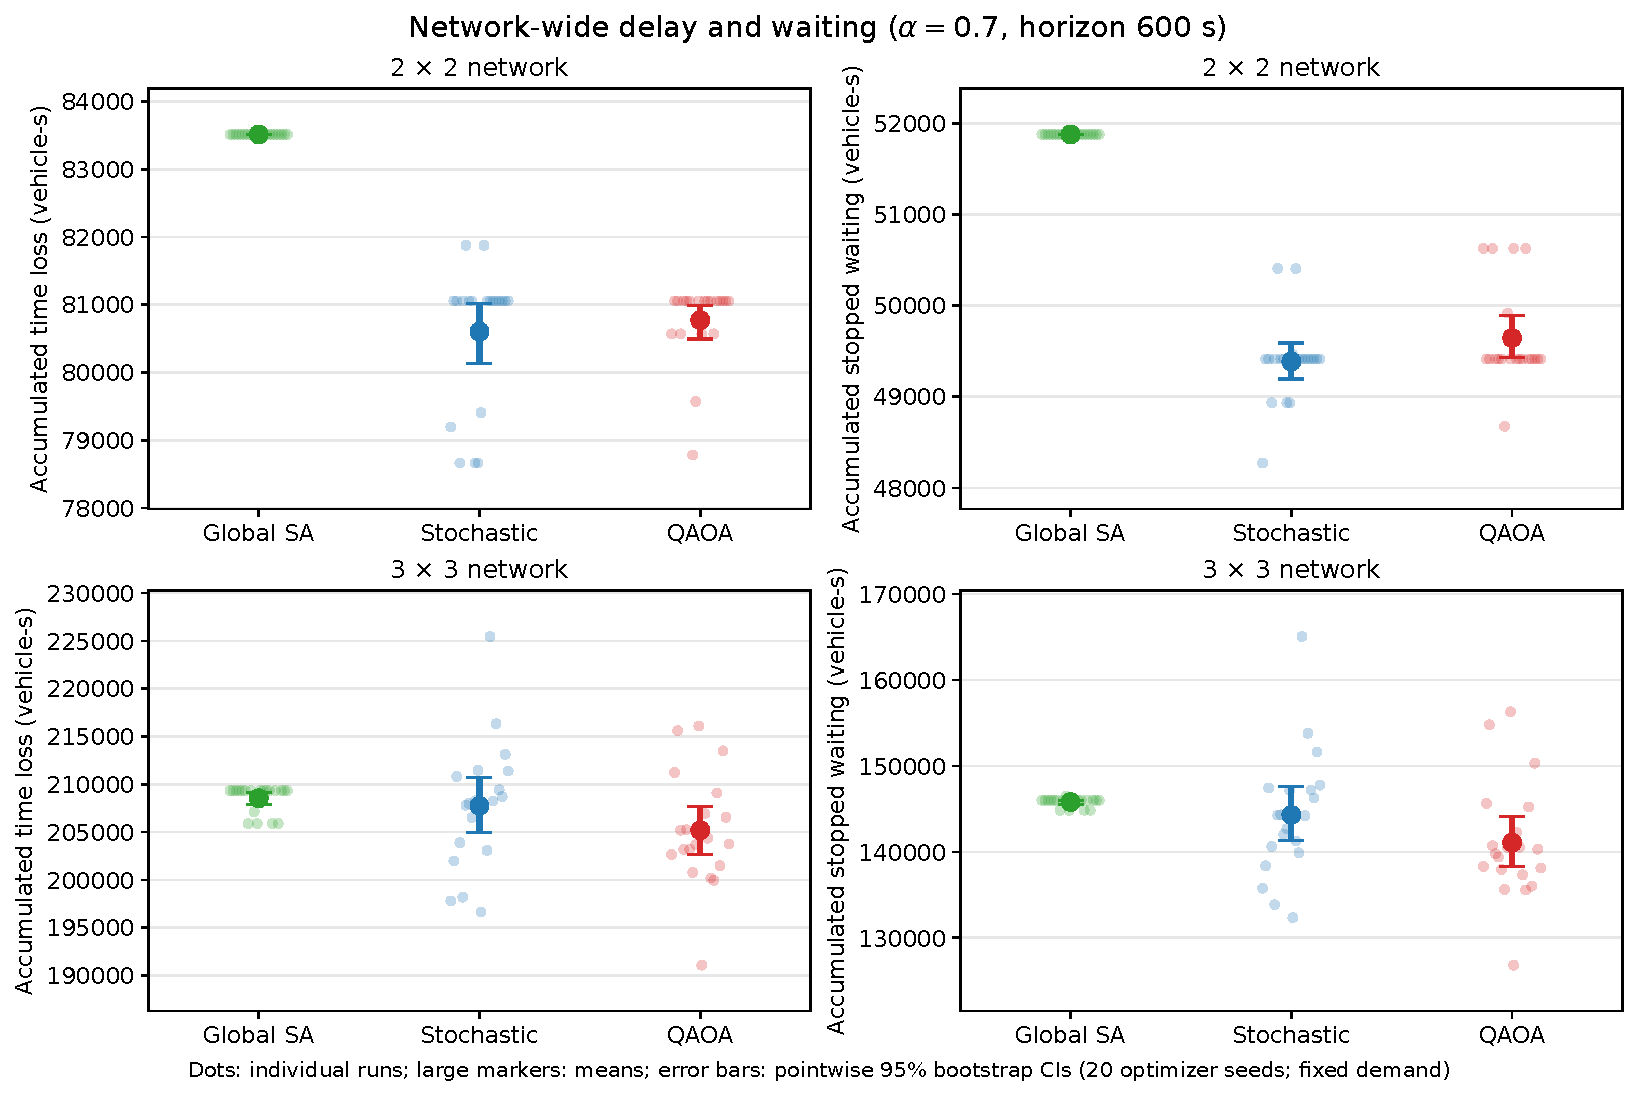
\includegraphics[width=\linewidth]{graphs/reviewer_population_accounting/figure_network_delay.pdf}
\caption{Accumulated network-wide time loss and stopped waiting, including completed, unfinished, and any removed vehicles through the cutoff. Vehicles awaiting insertion are excluded and reported separately. All conditions use $\alpha=0.7$ and fixed demand. Small dots show individual optimizer runs; large markers show means and error bars show pointwise 95\% percentile-bootstrap confidence intervals across 20 optimizer runs. These are not confidence intervals for controller differences.}
\label{fig:supplementary-network-delay}
\end{figure}

\begin{figure}[tbp]
\centering
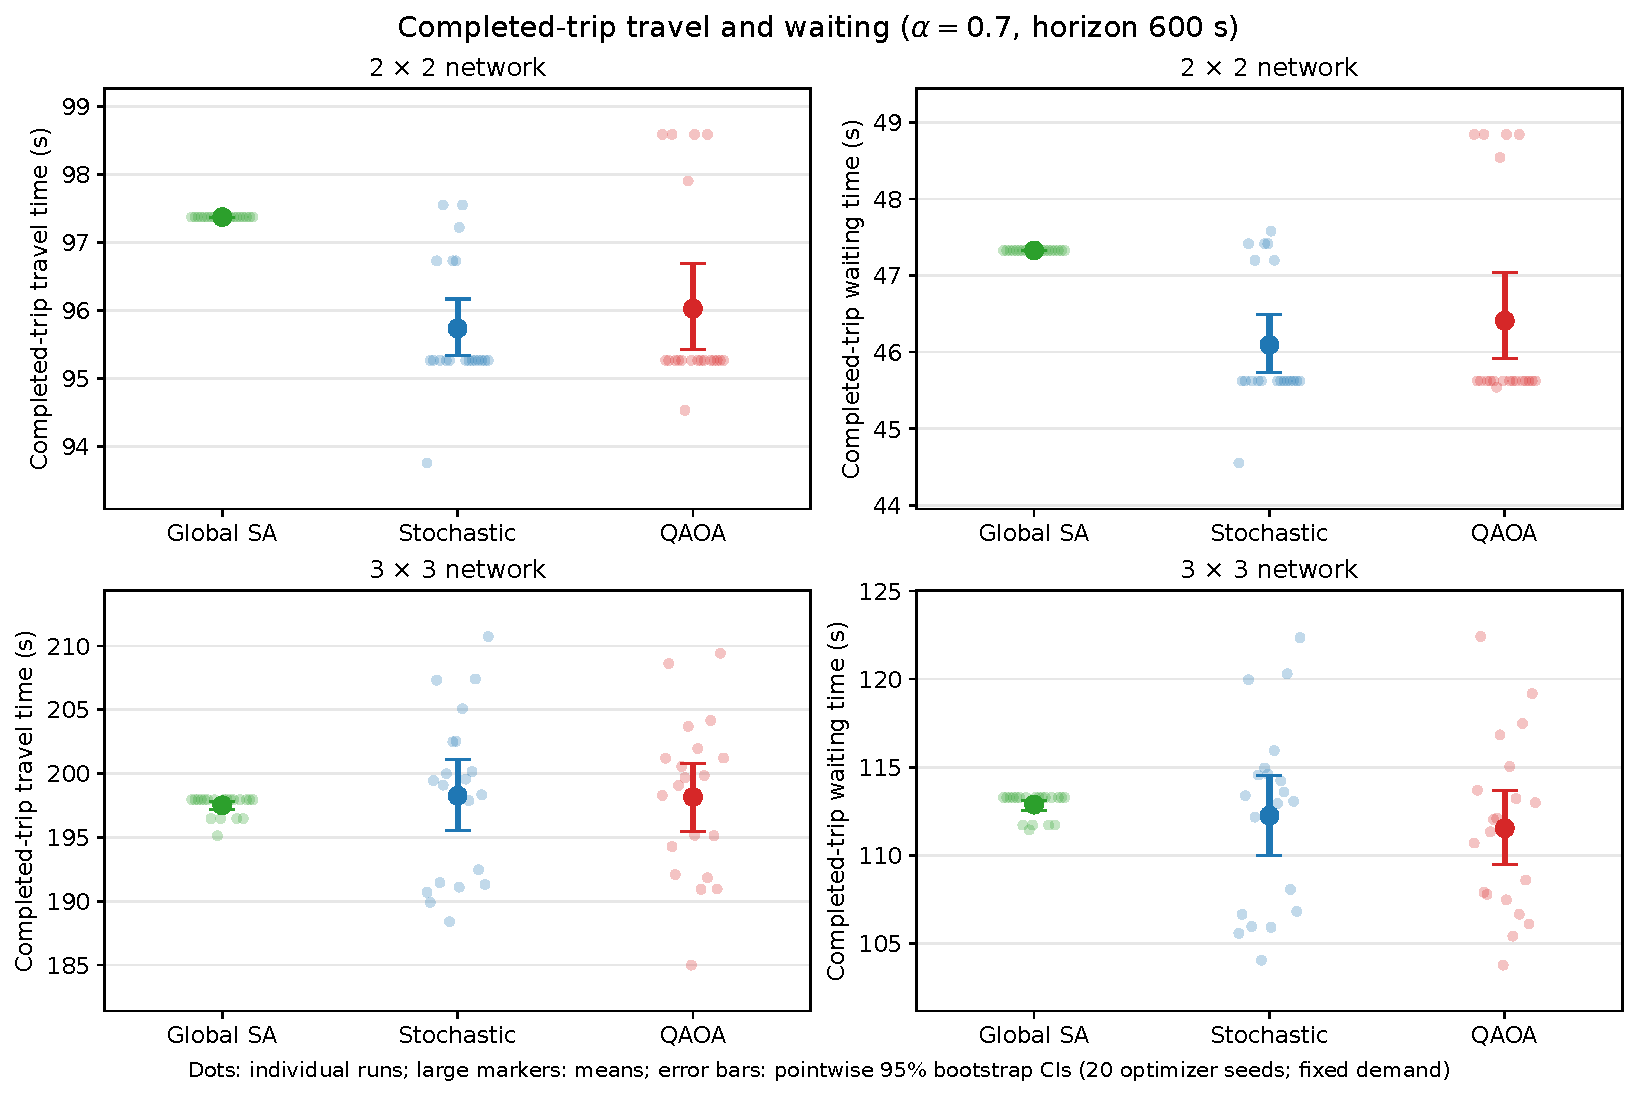
\includegraphics[width=\linewidth]{graphs/reviewer_population_accounting/figure_trip_times.pdf}
\caption{Completed-trip travel and waiting times. These averages are interpreted alongside population and network-wide delay accounting. All conditions use $\alpha=0.7$ and fixed demand. Small dots show individual optimizer runs; large markers show means and error bars show pointwise 95\% percentile-bootstrap confidence intervals across 20 optimizer runs. These are not confidence intervals for controller differences.}
\label{fig:supplementary-trip-times}
\end{figure}

\begin{figure}[tbp]
\centering
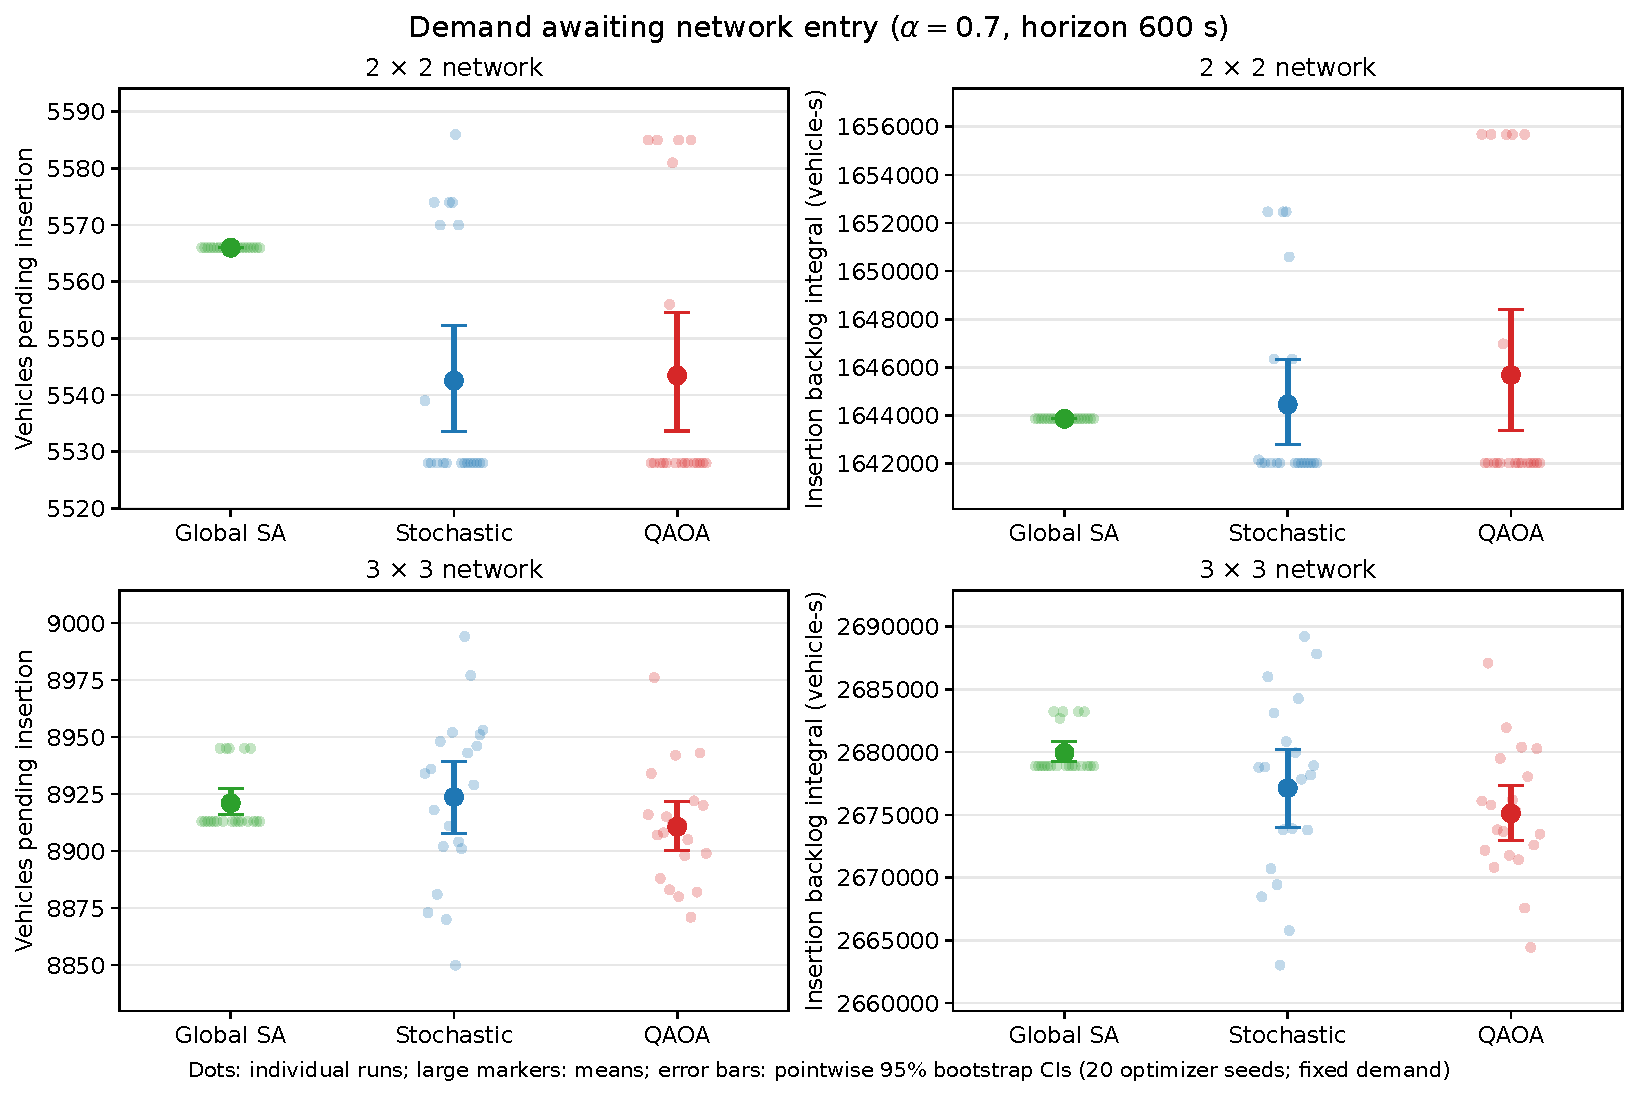
\includegraphics[width=\linewidth]{graphs/reviewer_population_accounting/figure_insertion_backlog.pdf}
\caption{Vehicles pending insertion at the cutoff and accumulated insertion backlog, measured as a discrete right-endpoint integral. These quantities are separate from in-network time loss. All conditions use $\alpha=0.7$ and fixed demand. Small dots show individual optimizer runs; large markers show means and error bars show pointwise 95\% percentile-bootstrap confidence intervals across 20 optimizer runs. These are not confidence intervals for controller differences.}
\label{fig:supplementary-insertion-backlog}
\end{figure}

